\section{ROS} \label{sec:ros}

ROS (Robot Operating System) es un conjunto de bibliotecas y herramientas que permiten desarrollar software para robots de manera modular y eficiente. Aunque su nombre sugiere que es un sistema operativo, en realidad funciona como una capa intermedia sobre un sistema operativo tradicional, como Ubuntu Linux. Esta capa facilita la integración de software complejo a través de herramientas y bibliotecas estandarizadas.

ROS admite lenguajes de programación como C++ y Python, lo que proporciona flexibilidad a los desarrolladores en la creación de algoritmos de control, procesamiento de datos y comunicación entre componentes. Ofrece desde funciones de bajo nivel, como controladores de hardware, hasta utilidades avanzadas de simulación, visualización y planificación de movimiento.

Fue desarrollado originalmente en el Laboratorio de Inteligencia Artificial de la Universidad de Stanford, y su mantenimiento ha sido continuado por la organización Open Robotics, responsable de su evolución y de versiones más recientes como ROS 2. ROS cuenta con diversos casos de uso como por ejemplo, se pueden cargar modelos URDF (Unified Robot Description Format) para visualizar y simular robots en entornos 3D, realizar pruebas de trayectorias, planificación de movimiento o pruebas de visión por computadora tal como se utilizó en nuestro proyecto. 

\begin{figure}[h]
	\centering
	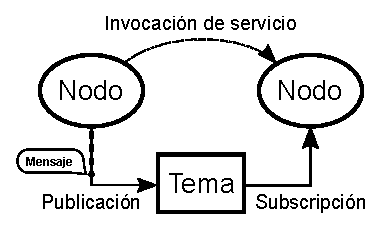
\includegraphics[width=0.5\linewidth]{img/ROS_concepts}
	\caption{Diagrama de comunicación de ROS}
	\label{fig:rosconcepts}
\end{figure}



\subsection{Nodo (Node)}

En el contexto de ROS, un nodo es una unidad básica de ejecución que representa un proceso individual dentro del sistema robótico. Cada nodo se encarga de realizar una tarea específica, como leer sensores, controlar actuadores o procesar datos.

Los nodos se comunican entre sí mediante una arquitectura distribuida, lo que permite que múltiples funciones se ejecuten simultáneamente de forma modular y eficiente. Esta comunicación se realiza principalmente a través de temas (topics) y servicios (services), que permiten el intercambio de información en tiempo real.

El uso de nodos independientes facilita el diseño, mantenimiento y escalabilidad del software, ya que cada nodo puede ser desarrollado, probado y ejecutado por separado.

\subsection{Tema (Topic)}

En ROS, un tema (topic) es un canal con nombre que permite la comunicación asíncrona entre nodos mediante el intercambio de mensajes. Este sistema está basado en un modelo de publicación-suscripción, en el cual un nodo puede publicar datos sobre un tema específico, mientras que uno o varios nodos pueden suscribirse a dicho tema para recibir la información correspondiente.

Esta arquitectura es especialmente útil para transmitir datos que se generan de manera continua, como lecturas de sensores, imágenes captadas por cámaras o la posición y velocidad actual del robot. Al ser una comunicación desacoplada, los nodos emisores y receptores no necesitan conocerse directamente, lo que mejora la modularidad y escalabilidad del sistema.

\subsection{Mensaje (Message)}

En ROS, un mensaje es una estructura de datos que se transmite entre nodos a través de los temas (topics). Representa la unidad básica de comunicación dentro del sistema. Estos mensajes pueden contener datos de tipo simple, como enteros, números flotantes o cadenas de texto, así como estructuras más complejas como arreglos, matrices o representaciones espaciales de coordenadas y orientaciones.

Cada tipo de mensaje está definido en un archivo `.msg`, donde se especifican los campos y tipos de datos que lo componen. Gracias a esta estandarización, los nodos pueden interpretar de manera correcta la información que reciben o envían, lo que facilita la interoperabilidad entre distintos componentes del sistema robótico.

\subsection{Servicio (Service)}

Un servicio en ROS es un mecanismo de comunicación basado en el modelo de solicitud-respuesta entre dos nodos. Este patrón permite que un nodo, denominado cliente de servicio, envíe una solicitud a otro nodo, llamado servidor de servicio, el cual ejecuta una tarea específica y devuelve una respuesta.

A diferencia de los temas, que funcionan de manera continua y asíncrona, los servicios se emplean para operaciones puntuales que requieren una interacción directa, como encender o apagar un dispositivo, ejecutar una acción determinada o solicitar un dato específico del sistema. Cada servicio está definido por un archivo `.srv` que especifica el tipo de datos de la solicitud y de la respuesta.

\subsection{Gazebo}

Gazebo es un entorno de simulación tridimensional que permite modelar y probar robots con alta precisión y realismo. Es compatible con ROS, lo cual permite una integración directa entre los nodos desarrollados y el entorno simulado. Este simulador proporciona herramientas para representar colisiones, aplicar fuerzas, simular sensores y realizar interacciones físicas con objetos del entorno, facilitando así la validación de algoritmos de control, percepción y navegación sin necesidad de utilizar hardware real.

Gracias a esta integración, los desarrolladores pueden evaluar el comportamiento de sus sistemas robóticos en diferentes escenarios y condiciones antes de implementarlos en plataformas físicas, optimizando tanto el desarrollo como la seguridad del robot.

\subsection{RViz}

RViz es una interfaz gráfica de visualización en ROS que permite representar en tiempo real los datos generados por los nodos del sistema robótico. Esta herramienta facilita la interpretación de información como mapas obtenidos mediante sensores LIDAR, modelos tridimensionales del robot, trayectorias planificadas y su posición en el espacio.

Gracias a sus capacidades gráficas, RViz se convierte en una herramienta fundamental para el análisis, depuración y supervisión del comportamiento del robot durante su operación. Su uso es clave tanto en la fase de desarrollo como en la validación de algoritmos y sistemas dentro del entorno ROS.
